

% IEEEtran V1.7 and later provides for these CLASSINPUT macros to allow the
% user to reprogram some IEEEtran.cls defaults if needed. These settings
% override the internal defaults of IEEEtran.cls regardless of which class
% options are used. Do not use these unless you have good reason to do so as
% they can result in nonIEEE compliant documents. User beware. ;)
%
%\newcommand{\CLASSINPUTbaselinestretch}{1.0} % baselinestretch
%\newcommand{\CLASSINPUTinnersidemargin}{1in} % inner side margin
%\newcommand{\CLASSINPUToutersidemargin}{1in} % outer side margin
%\newcommand{\CLASSINPUTtoptextmargin}{1in}   % top text margin
%\newcommand{\CLASSINPUTbottomtextmargin}{1in}% bottom text margin


% Note that the a4paper option is mainly intended so that authors in
% countries using A4 can easily print to A4 and see how their papers will
% look in print - the typesetting of the document will not typically be
% affected with changes in paper size (but the bottom and side margins will).
% Use the testflow package mentioned above to verify correct handling of
% both paper sizes by the user's LaTeX system.
%
% Also note that the "draftcls" or "draftclsnofoot", not "draft", option
% should be used if it is desired that the figures are to be displayed in
% draft mode.
%
\documentclass[11pt, conference, compsoc]{IEEEtran}
% The Computer Society requires 12pt.
% If IEEEtran.cls has not been installed into the LaTeX system files,
% manually specify the path to it like:
% \documentclass[10pt,journal,compsoc]{../sty/IEEEtran}


% For Computer Society journals, IEEEtran defaults to the use of 
% Palatino/Palladio as is done in IEEE Computer Society journals.
% To go back to Times Roman, you can use this code:
%\renewcommand{\rmdefault}{ptm}\selectfont

\usepackage{amsmath}
\usepackage{algorithm}
\usepackage[noend]{algpseudocode}

\makeatletter
\def\BState{\State\hskip-\ALG@thistlm}
\makeatother



% Some very useful LaTeX packages include:
% (uncomment the ones you want to load)



% *** MISC UTILITY PACKAGES ***
%
%\usepackage{ifpdf}
% Heiko Oberdiek's ifpdf.sty is very useful if you need conditional
% compilation based on whether the output is pdf or dvi.
% usage:
% \ifpdf
%   % pdf code
% \else
%   % dvi code
% \fi
% The latest version of ifpdf.sty can be obtained from:
% http://www.ctan.org/tex-archive/macros/latex/contrib/oberdiek/
% Also, note that IEEEtran.cls V1.7 and later provides a builtin
% \ifCLASSINFOpdf conditional that works the same way.
% When switching from latex to pdflatex and vice-versa, the compiler may
% have to be run twice to clear warning/error messages.



%\usepackage{natbib}
\usepackage{cite}
\usepackage{placeins}
% *** CITATION PACKAGES ***
%
%\ifCLASSOPTIONcompsoc
  % IEEE Computer Society needs nocompress option
  % requires cite.sty v4.0 or later (November 2003)
%   \usepackage[nocompress]{cite}
%\else
  % normal IEEE
%   \usepackage{cite}
%\fi

% cite.sty was written by Donald Arseneau
% V1.6 and later of IEEEtran pre-defines the format of the cite.sty package
% \cite{} output to follow that of IEEE. Loading the cite package will
% result in citation numbers being automatically sorted and properly
% "compressed/ranged". e.g., [1], [9], [2], [7], [5], [6] without using
% cite.sty will become [1], [2], [5]--[7], [9] using cite.sty. cite.sty's
% \cite will automatically add leading space, if needed. Use cite.sty's
% noadjust option (cite.sty V3.8 and later) if you want to turn this off.
% cite.sty is already installed on most LaTeX systems. Be sure and use
% version 4.0 (2003-05-27) and later if using hyperref.sty. cite.sty does
% not currently provide for hyperlinked citations.
% The latest version can be obtained at:
% http://www.ctan.org/tex-archive/macros/latex/contrib/cite/
% The documentation is contained in the cite.sty file itself.
%
% Note that some packages require special options to format as the Computer
% Society requires. In particular, Computer Society  papers do not use
% compressed citation ranges as is done in typical IEEE papers
% (e.g., [1]-[4]). Instead, they list every citation separately in order
% (e.g., [1], [2], [3], [4]). To get the latter we need to load the cite
% package with the nocompress option which is supported by cite.sty v4.0
% and later. Note also the use of a CLASSOPTION conditional provided by
% IEEEtran.cls V1.7 and later.





% *** GRAPHICS RELATED PACKAGES ***
%
\usepackage[pdftex]{graphicx}
\ifCLASSINFOpdf
  % \usepackage[pdftex]{graphicx}
  % declare the path(s) where your graphic files are
  % \graphicspath{{../pdf/}{../jpeg/}}
  % and their extensions so you won't have to specify these with
  % every instance of \includegraphics
  % \DeclareGraphicsExtensions{.pdf,.jpeg,.png}
\else
  % or other class option (dvipsone, dvipdf, if not using dvips). graphicx
  % will default to the driver specified in the system graphics.cfg if no
  % driver is specified.
  % \usepackage[dvips]{graphicx}
  % declare the path(s) where your graphic files are
  % \graphicspath{{../eps/}}
  % and their extensions so you won't have to specify these with
  % every instance of \includegraphics
  % \DeclareGraphicsExtensions{.eps}
\fi
% graphicx was written by David Carlisle and Sebastian Rahtz. It is
% required if you want graphics, photos, etc. graphicx.sty is already
% installed on most LaTeX systems. The latest version and documentation can
% be obtained at: 
% http://www.ctan.org/tex-archive/macros/latex/required/graphics/
% Another good source of documentation is "Using Imported Graphics in
% LaTeX2e" by Keith Reckdahl which can be found as epslatex.ps or
% epslatex.pdf at: http://www.ctan.org/tex-archive/info/
%
% latex, and pdflatex in dvi mode, support graphics in encapsulated
% postscript (.eps) format. pdflatex in pdf mode supports graphics
% in .pdf, .jpeg, .png and .mps (metapost) formats. Users should ensure
% that all non-photo figures use a vector format (.eps, .pdf, .mps) and
% not a bitmapped formats (.jpeg, .png). IEEE frowns on bitmapped formats
% which can result in "jaggedy"/blurry rendering of lines and letters as
% well as large increases in file sizes.
%
% You can find documentation about the pdfTeX application at:
% http://www.tug.org/applications/pdftex



%\usepackage{ps4pdf}
% dvi->ps workflow is required to use such packages as psfrag.sty and
% pstricks.sty. However, Rolf Niepraschk's ps4pdf.sty provides a way to
% apply psfrag/pstricks effects to .eps figures and then get the resultant
% figures in .pdf form. Thus, providing an easier way for migrating from
% .eps to .pdf figures. After ps4pdf.sty loads, if:
% 1. producing .dvi output: the output file will consist ONLY of the
%    figures (or other constructs encased within \PSforPDF commands)
% 2. producing .pdf output: pdflatex will look in the filename-pics.pdf
%    file, where filename is the basename of the tex document, for the
%    graphics (or other constructs encased within \PSforPDF commands).
%    NOTE: If you ever change your figures, you must remember to remake
%    the filename-pics.pdf file.
%
% This way you can do a:
% 
% latex filename
% dvips -Ppdf -o filename-pics.ps filename.dvi
% ps2pdf filename-pics.ps filename-pics.pdf
% 
% to produce a filename-pics.pdf graphics container that contains
% .pdf versions of the graphics with psfrag, pstricks, etc. features.
% Note that you will not typically be able to view the figures in 
% filename-pics.ps because of an offset. However, you will be able to
% view them in filename-pics.pdf. Also, note that when ps4pdf is in effect
% with .dvi output, you may get harmless over/under full box warnings - 
% ignore them. 
% Then, run pdflatex:
% 
% pdflatex filename
% 
% to use pdflatex to make PDF output, automatically using the figures in
% filename-pics.pdf. Alternatively, you could use dvips -i option to
% obtain separate .pdf files for each figure:
%
% dvips -Ppdf -i -E -o fig filename
%
% then convert each figure to pdf via a command such as epstopdf and then
% use pdflatex with these pdf figures and then to dispense with ps4pdf.
%
% Remember to rerun through latex/dvips/ps2pdf if you ever change your
% figures so that filename-pics.pdf gets updated.
% ps4pdf requires David Kastrup's preview-latex and a recent LaTeX system
% (circa 2001 or later). The ps4pdf package and documentation can be
% obtained at: http://www.ctan.org/tex-archive/macros/latex/contrib/ps4pdf/
% The preview-latex package and documentation can be obtained at:
% http://www.ctan.org/tex-archive/macros/latex/contrib/preview/
%
% provide a bogus \PSforPDF, even when not loading pd4pdf. This way we can
% stop loading ps4pdf.sty if we choose to make separate .pdf versions of
% each of our figures.
\providecommand{\PSforPDF}[1]{#1}
% Note that in order for ps4pdf to work, all commands related to psfrag,
% pstricks, etc. must be called within the PSforPDF command. This applies
% even when *loading* via \usepackage psfrag.sty, etc.


%\PSforPDF{\usepackage{psfrag}}
% psfrag.sty was written by Craig Barratt, Michael C. Grant, and
% David Carlisle. It allows you to substitute LaTeX commands for text in
% imported EPS graphic files. In this way, LaTeX symbols can be placed into
% graphics that have been generated by other applications. You must use
% latex->dvips->ps2pdf workflow (not direct pdf output from pdflatex) if
% you wish to use this capability because it works via some PostScript
% tricks. Alternatively, the graphics could be processed as separate files
% via psfrag and dvips, then converted to PDF for inclusion in the main file
% which uses pdflatex. ps4pdf.sty (above) provides a way of doing this all
% at once within the main file.
% Docs are in "The PSfrag System" by Michael C. Grant and David Carlisle.
% There is also some information about using psfrag in "Using Imported
% Graphics in LaTeX2e" by Keith Reckdahl which documents the graphicx
% package (see above). The psfrag package and documentation can be obtained
% at: http://www.ctan.org/tex-archive/macros/latex/contrib/psfrag/
% 
% Note that the current version of psfrag does not "turn itself off" when
% running under pdf output. This will result in a harmless warning
% about a non-PDF \special. However, to silence this, a bogus psfrag
% command can be provided instead of loading psfrag.sty when PDF output
% is being used. Thus, a more complex alternative conditional loading scheme
% can be employed instead of the straightforword way above:
%
%\ifCLASSINFOpdf
% if outputting PDF, do not use or load psfrag.sty as current versions
% output a non-PDF special that generates a harmless, but annoying warning.
% Instead, we provide a bogus \psfrag command that does nothing with
% its arguments. This is a tad tricky because \psfrag can have up to six
% arguments four of which are optional: \psfrag{}[][][][]{}
% Code based on that in psfrag.sty
%\makeatletter
%\def\psfrag{\@ifstar{\@BOGUSpsfraga}{\@BOGUSpsfraga}}
%\def\@BOGUSpsfraga{\begingroup
%   \@makeother\"\@makeother\*\@makeother\!\@makeother\~%
%   \@makeother\:\@makeother\\\@makeother\%\@makeother\#%
%   \@makeother\ \@BOGUSpsfragb}
%\def\@BOGUSpsfragb#1{\endgroup
%                \@ifnextchar [{\@BOGUSpsfragc}%
%                              {\@BOGUSpsfrag}}
%\def\@BOGUSpsfragc[#1]{\@ifnextchar [{\@BOGUSpsfragd}%
%                                     {\@BOGUSpsfrag}}
%\def\@BOGUSpsfragd[#1]{\@ifnextchar [{\@BOGUSpsfrage}%
%                                     {\@BOGUSpsfrag}}
%\def\@BOGUSpsfrage[#1]{\@ifnextchar [{\@BOGUSpsfragf}%
%                                     {\@BOGUSpsfrag}}
%\def\@BOGUSpsfragf[#1]{\@BOGUSpsfrag}
%\def\@BOGUSpsfrag#1{\ignorespaces}
%\makeatother
%\else
% using dvi output, load psfrag, but funnel it through PSforPDF
% as required by ps4pdf.sty
%\PSforPDF{\usepackage{psfrag}}
%\fi





% *** MATH PACKAGES ***
%
%\usepackage[cmex10]{amsmath}
% A popular package from the American Mathematical Society that provides
% many useful and powerful commands for dealing with mathematics. If using
% it, be sure to load this package with the cmex10 option to ensure that
% only type 1 fonts will utilized at all point sizes. Without this option,
% it is possible that some math symbols, particularly those within
% footnotes, will be rendered in bitmap form which will result in a
% document that can not be IEEE Xplore compliant!
%
% Also, note that the amsmath package sets \interdisplaylinepenalty to 10000
% thus preventing page breaks from occurring within multiline equations. Use:
%\interdisplaylinepenalty=2500
% after loading amsmath to restore such page breaks as IEEEtran.cls normally
% does. amsmath.sty is already installed on most LaTeX systems. The latest
% version and documentation can be obtained at:
% http://www.ctan.org/tex-archive/macros/latex/required/amslatex/math/





% *** SPECIALIZED LIST PACKAGES ***
%\usepackage{acronym}
% acronym.sty was written by Tobias Oetiker. This package provides tools for
% managing documents with large numbers of acronyms. (You don't *have* to
% use this package - unless you have a lot of acronyms, you may feel that
% such package management of them is bit of an overkill.)
% Do note that the acronym environment (which lists acronyms) will have a
% problem when used under IEEEtran.cls because acronym.sty relies on the
% description list environment - which IEEEtran.cls has customized for
% producing IEEE style lists. A workaround is to declared the longest
% label width via the IEEEtran.cls \IEEEiedlistdecl global control:
%
% \renewcommand{\IEEEiedlistdecl}{\IEEEsetlabelwidth{SONET}}
% \begin{acronym}
%
% \end{acronym}
% \renewcommand{\IEEEiedlistdecl}{\relax}% remember to reset \IEEEiedlistdecl
%
% instead of using the acronym environment's optional argument.
% The latest version and documentation can be obtained at:
% http://www.ctan.org/tex-archive/macros/latex/contrib/acronym/


%\usepackage{algorithmic}
% algorithmic.sty was written by Peter Williams and Rogerio Brito.
% This package provides an algorithmic environment fo describing algorithms.
% You can use the algorithmic environment in-text or within a figure
% environment to provide for a floating algorithm. Do NOT use the algorithm
% floating environment provided by algorithm.sty (by the same authors) or
% algorithm2e.sty (by Christophe Fiorio) as IEEE does not use dedicated
% algorithm float types and packages that provide these will not provide
% correct IEEE style captions. The latest version and documentation of
% algorithmic.sty can be obtained at:
% http://www.ctan.org/tex-archive/macros/latex/contrib/algorithms/
% There is also a support site at:
% http://algorithms.berlios.de/index.html
% Also of interest may be the (relatively newer and more customizable)
% algorithmicx.sty package by Szasz Janos:
% http://www.ctan.org/tex-archive/macros/latex/contrib/algorithmicx/




% *** ALIGNMENT PACKAGES ***
%
%\usepackage{array}
% Frank Mittelbach's and David Carlisle's array.sty patches and improves
% the standard LaTeX2e array and tabular environments to provide better
% appearance and additional user controls. As the default LaTeX2e table
% generation code is lacking to the point of almost being broken with
% respect to the quality of the end results, all users are strongly
% advised to use an enhanced (at the very least that provided by array.sty)
% set of table tools. array.sty is already installed on most systems. The
% latest version and documentation can be obtained at:
% http://www.ctan.org/tex-archive/macros/latex/required/tools/


%\usepackage{mdwmath}
%\usepackage{mdwtab}
% Also highly recommended is Mark Wooding's extremely powerful MDW tools,
% especially mdwmath.sty and mdwtab.sty which are used to format equations
% and tables, respectively. The MDWtools set is already installed on most
% LaTeX systems. The lastest version and documentation is available at:
% http://www.ctan.org/tex-archive/macros/latex/contrib/mdwtools/


% IEEEtran contains the IEEEeqnarray family of commands that can be used to
% generate multiline equations as well as matrices, tables, etc., of high
% quality.


%\usepackage{eqparbox}
% Also of notable interest is Scott Pakin's eqparbox package for creating
% (automatically sized) equal width boxes - aka "natural width parboxes".
% Available at:
% http://www.ctan.org/tex-archive/macros/latex/contrib/eqparbox/





% *** SUBFIGURE PACKAGES ***
\ifCLASSOPTIONcompsoc
\usepackage[tight,normalsize,sf,SF]{subfigure}
\else
\usepackage[tight,footnotesize]{subfigure}
\fi
% subfigure.sty was written by Steven Douglas Cochran. This package makes it
% easy to put subfigures in your figures. e.g., "Figure 1a and 1b". For IEEE
% work, it is a good idea to load it with the tight package option to reduce
% the amount of white space around the subfigures. Computer Society papers
% use a larger font and \sffamily font for their captions, hence the
% additional options needed under compsoc mode. subfigure.sty is already
% installed on most LaTeX systems. The latest version and documentation can
% be obtained at:
% http://www.ctan.org/tex-archive/obsolete/macros/latex/contrib/subfigure/
% subfigure.sty has been superceeded by subfig.sty.


%\ifCLASSOPTIONcompsoc
%  \usepackage[caption=false]{caption}
%  \usepackage[font=normalsize,labelfont=sf,textfont=sf]{subfig}
%\else
%  \usepackage[caption=false]{caption}
%  \usepackage[font=footnotesize]{subfig}
%\fi
% subfig.sty, also written by Steven Douglas Cochran, is the modern
% replacement for subfigure.sty. However, subfig.sty requires and
% automatically loads Axel Sommerfeldt's caption.sty which will override
% IEEEtran.cls handling of captions and this will result in nonIEEE style
% figure/table captions. To prevent this problem, be sure and preload
% caption.sty with its "caption=false" package option. This is will preserve
% IEEEtran.cls handing of captions. Version 1.3 (2005/06/28) and later 
% (recommended due to many improvements over 1.2) of subfig.sty supports
% the caption=false option directly:
\ifCLASSOPTIONcompsoc
  \usepackage[caption=false,font=normalsize,labelfont=sf,textfont=sf]{subfig}
\else
  \usepackage[caption=false,font=footnotesize]{subfig}
\fi
%
% The latest version and documentation can be obtained at:
% http://www.ctan.org/tex-archive/macros/latex/contrib/subfig/
% The latest version and documentation of caption.sty can be obtained at:
% http://www.ctan.org/tex-archive/macros/latex/contrib/caption/




% *** FLOAT PACKAGES ***
%
%\usepackage{fixltx2e}
% fixltx2e, the successor to the earlier fix2col.sty, was written by
% Frank Mittelbach and David Carlisle. This package corrects a few problems
% in the LaTeX2e kernel, the most notable of which is that in current
% LaTeX2e releases, the ordering of single and double column floats is not
% guaranteed to be preserved. Thus, an unpatched LaTeX2e can allow a
% single column figure to be placed prior to an earlier double column
% figure. The latest version and documentation can be found at:
% http://www.ctan.org/tex-archive/macros/latex/base/


%\usepackage{stfloats}
% stfloats.sty was written by Sigitas Tolusis. This package gives LaTeX2e
% the ability to do double column floats at the bottom of the page as well
% as the top. (e.g., "\begin{figure*}[!b]" is not normally possible in
% LaTeX2e). It also provides a command:
%\fnbelowfloat
% to enable the placement of footnotes below bottom floats (the standard
% LaTeX2e kernel puts them above bottom floats). This is an invasive package
% which rewrites many portions of the LaTeX2e float routines. It may not work
% with other packages that modify the LaTeX2e float routines. The latest
% version and documentation can be obtained at:
% http://www.ctan.org/tex-archive/macros/latex/contrib/sttools/
% Documentation is contained in the stfloats.sty comments as well as in the
% presfull.pdf file. Do not use the stfloats baselinefloat ability as IEEE
% does not allow \baselineskip to stretch. Authors submitting work to the
% IEEE should note that IEEE rarely uses double column equations and
% that authors should try to avoid such use. Do not be tempted to use the
% cuted.sty or midfloat.sty packages (also by Sigitas Tolusis) as IEEE does
% not format its papers in such ways.


\ifCLASSOPTIONcaptionsoff
  \usepackage[nomarkers]{endfloat}
 \let\MYoriglatexcaption\caption
 \renewcommand{\caption}[2][\relax]{\MYoriglatexcaption[#2]{#2}}
\fi
% endfloat.sty was written by James Darrell McCauley and Jeff Goldberg.
% This package may be useful when used in conjunction with IEEEtran.cls'
% captionsoff option. Some IEEE journals/societies require that submissions
% have lists of figures/tables at the end of the paper and that
% figures/tables without any captions are placed on a page by themselves at
% the end of the document. If needed, the draftcls IEEEtran class option or
% \CLASSINPUTbaselinestretch interface can be used to increase the line
% spacing as well. Be sure and use the nomarkers option of endfloat to
% prevent endfloat from "marking" where the figures would have been placed
% in the text. The two hack lines of code above are a slight modification of
% that suggested by in the endfloat docs (section 8.3.1) to ensure that
% the full captions always appear in the list of figures/tables - even if
% the user used the short optional argument of \caption[]{}.
% IEEE papers do not typically make use of \caption[]'s optional argument,
% so this should not be an issue. A similar trick can be used to disable
% captions of packages such as subfig.sty that lack options to turn off
% the subcaptions:
% For subfig.sty:
% \let\MYorigsubfloat\subfloat
% \renewcommand{\subfloat}[2][\relax]{\MYorigsubfloat[]{#2}}
% For subfigure.sty:
% \let\MYorigsubfigure\subfigure
% \renewcommand{\subfigure}[2][\relax]{\MYorigsubfigure[]{#2}}
% However, the above trick will not work if both optional arguments of
% the \subfloat/subfig command are used. Furthermore, there needs to be a
% description of each subfigure *somewhere* and endfloat does not add
% subfigure captions to its list of figures. Thus, the best approach is to
% avoid the use of subfigure captions (many IEEE journals avoid them anyway)
% and instead reference/explain all the subfigures within the main caption.
% The latest version of endfloat.sty and its documentation can obtained at:
% http://www.ctan.org/tex-archive/macros/latex/contrib/endfloat/
%
% The IEEEtran \ifCLASSOPTIONcaptionsoff conditional can also be used
% later in the document, say, to conditionally put the References on a 
% page by themselves.





% *** PDF, URL AND HYPERLINK PACKAGES ***
%
%\usepackage{url}
% url.sty was written by Donald Arseneau. It provides better support for
% handling and breaking URLs. url.sty is already installed on most LaTeX
% systems. The latest version can be obtained at:
% http://www.ctan.org/tex-archive/macros/latex/contrib/misc/
% Read the url.sty source comments for usage information. Basically,
% \url{my_url_here}.


% NOTE: PDF thumbnail features are not required in IEEE papers
%       and their use requires extra complexity and work.
%\ifCLASSINFOpdf
%  \usepackage[pdftex]{thumbpdf}
%\else
%  \usepackage[dvips]{thumbpdf}
%\fi
% thumbpdf.sty and its companion Perl utility were written by Heiko Oberdiek.
% It allows the user a way to produce PDF documents that contain fancy
% thumbnail images of each of the pages (which tools like acrobat reader can
% utilize). This is possible even when using dvi->ps->pdf workflow if the
% correct thumbpdf driver options are used. thumbpdf.sty incorporates the
% file containing the PDF thumbnail information (filename.tpm is used with
% dvips, filename.tpt is used with pdftex, where filename is the base name of
% your tex document) into the final ps or pdf output document. An external
% utility, the thumbpdf *Perl script* is needed to make these .tpm or .tpt
% thumbnail files from a .ps or .pdf version of the document (which obviously
% does not yet contain pdf thumbnails). Thus, one does a:
% 
% thumbpdf filename.pdf 
%
% to make a filename.tpt, and:
%
% thumbpdf --mode dvips filename.ps
%
% to make a filename.tpm which will then be loaded into the document by
% thumbpdf.sty the NEXT time the document is compiled (by pdflatex or
% latex->dvips->ps2pdf). Users must be careful to regenerate the .tpt and/or
% .tpm files if the main document changes and then to recompile the
% document to incorporate the revised thumbnails to ensure that thumbnails
% match the actual pages. It is easy to forget to do this!
% 
% Unix systems come with a Perl interpreter. However, MS Windows users
% will usually have to install a Perl interpreter so that the thumbpdf
% script can be run. The Ghostscript PS/PDF interpreter is also required.
% See the thumbpdf docs for details. The latest version and documentation
% can be obtained at.
% http://www.ctan.org/tex-archive/support/thumbpdf/
% Be sure and use only version 3.8 (2005/07/06) or later of thumbpdf as
% earlier versions will not work properly with recent versions of pdfTeX
% (1.20a and later).


% NOTE: PDF hyperlink and bookmark features are not required in IEEE
%       papers and their use requires extra complexity and work.
% *** IF USING HYPERREF BE SURE AND CHANGE THE EXAMPLE PDF ***
% *** TITLE/SUBJECT/AUTHOR/KEYWORDS INFO BELOW!!           ***
\newcommand\MYhyperrefoptions{bookmarks=true,bookmarksnumbered=true,
pdfpagemode={UseOutlines},plainpages=false,pdfpagelabels=true,
colorlinks=true,linkcolor={black},citecolor={black},pagecolor={black},
urlcolor={black},
pdftitle={Online adaptive content personalisation},%<!CHANGE!
pdfsubject={Markov decision processes},%<!CHANGE!
pdfauthor={Jonathan K. Wasson},%<!CHANGE!
pdfkeywords={MDP, content personalisation, machine learning}}%<^!CHANGE!
%\ifCLASSINFOpdf
%\usepackage[\MYhyperrefoptions,pdftex]{hyperref}
%\else
%\usepackage[\MYhyperrefoptions,breaklinks=true,dvips]{hyperref}
%\usepackage{breakurl}
%\fi
% One significant drawback of using hyperref under DVI output is that the
% LaTeX compiler cannot break URLs across lines or pages as can be done
% under pdfLaTeX's PDF output via the hyperref pdftex driver. This is
% probably the single most important capability distinction between the
% DVI and PDF output. Perhaps surprisingly, all the other PDF features
% (PDF bookmarks, thumbnails, etc.) can be preserved in
% .tex->.dvi->.ps->.pdf workflow if the respective packages/scripts are
% loaded/invoked with the correct driver options (dvips, etc.). 
% As most IEEE papers use URLs sparingly (mainly in the references), this
% may not be as big an issue as with other publications.
%
% That said, recently Vilar Camara Neto introduced his breakurl.sty
% package which permits hyperref to easily break URLs even in dvi
% mode. Note that breakurl, unlike most other packages, must be loaded
% AFTER hyperref. The latest version of breakurl and its documentation can
% be obtained at:
% http://www.ctan.org/tex-archive/macros/latex/contrib/breakurl/
% breakurl.sty is not for use under pdflatex pdf mode. Versions 1.10 
% (September 23, 2005) and later are recommened to avoid bugs in earlier
% releases.
%
% The advanced features offer by hyperref.sty are not required for IEEE
% submission, so users should weigh these features against the added
% complexity of use. Users who wish to use hyperref *must* ensure that
% their hyperref version is 6.72u or later *and* IEEEtran.cls is version
% 1.6b or later.
% The package options above demonstrate how to enable PDF bookmarks
% (a type of table of contents viewable in Acrobat Reader) as well as
% PDF document information (title, subject, author and keywords) that is
% viewable in Acrobat reader's Document_Properties menu. PDF document
% information is also used extensively to automate the cataloging of PDF
% documents. The above set of options ensures that hyperlinks will not be
% colored in the text and thus will not be visible in the printed page,
% but will be active on "mouse over". USING COLORS OR OTHER HIGHLIGHTING
% OF HYPERLINKS CAN RESULT IN DOCUMENT REJECTION BY THE IEEE, especially if
% these appear on the "printed" page. IF IN DOUBT, ASK THE RELEVANT
% SUBMISSION EDITOR. You may need to add the option hypertexnames=false if
% you used duplicate equation numbers, etc., but this should not be needed
% in normal IEEE work.
% The latest version of hyperref and its documentation can be obtained at:
% http://www.ctan.org/tex-archive/macros/latex/contrib/hyperref/





% *** Do not adjust lengths that control margins, column widths, etc. ***
% *** Do not use packages that alter fonts (such as pslatex).         ***
% There should be no need to do such things with IEEEtran.cls V1.6 and later.
% (Unless specifically asked to do so by the journal or conference you plan
% to submit to, of course. )


% correct bad hyphenation here
\hyphenation{op-tical net-works semi-conduc-tor}


\begin{document}
%
% paper title
% can use linebreaks \\ within to get better formatting as desired
\title{Towards Online Adaptive \\ Content Personalisation}
%
%
% author names and IEEE memberships
% note positions of commas and nonbreaking spaces ( ~ ) LaTeX will not break
% a structure at a ~ so this keeps an author's name from being broken across
% two lines.
% use \thanks{} to gain access to the first footnote area
% a separate \thanks must be used for each paragraph as LaTeX2e's \thanks
% was not built to handle multiple paragraphs
%
%
%\IEEEcompsocitemizethanks is a special \thanks that produces the bulleted
% lists the Computer Society journals use for "first footnote" author
% affiliations. Use \IEEEcompsocthanksitem which works much like \item
% for each affiliation group. When not in compsoc mode,
% \IEEEcompsocitemizethanks becomes like \thanks and
% \IEEEcompsocthanksitem becomes a line break with idention. This
% facilitates dual compilation, although admittedly the differences in the
% desired content of \author between the different types of papers makes a
% one-size-fits-all approach a daunting prospect. For instance, compsoc 
% journal papers have the author affiliations above the "Manuscript
% received ..."  text while in non-compsoc journals this is reversed. Sigh.

\author{\textbf{Jonathan~K.~Wasson}\\
School of Computer Science\\
University of the Witwatersrand\\
South Africa\\
wassonjonathan@gmail.com
\and
\textbf{Benjamin~Rosman}\\
School of Computer Science\\
University of the Witwatersrand\\
South Africa\\
benjros@gmail.com

}

% note the % following the last \IEEEmembership and also \thanks - 
% these prevent an unwanted space from occurring between the last author name
% and the end of the author line. i.e., if you had this:
% 
% \author{....lastname \thanks{...} \thanks{...} }
%                     ^------------^------------^----Do not want these spaces!
%
% a space would be appended to the last name and could cause every name on that
% line to be shifted left slightly. This is one of those "LaTeX things". For
% instance, "\textbf{A} \textbf{B}" will typeset as "A B" not "AB". To get
% "AB" then you have to do: "\textbf{A}\textbf{B}"
% \thanks is no different in this regard, so shield the last } of each \thanks
% that ends a line with a % and do not let a space in before the next \thanks.
% Spaces after \IEEEmembership other than the last one are OK (and needed) as
% you are supposed to have spaces between the names. For what it is worth,
% this is a minor point as most people would not even notice if the said evil
% space somehow managed to creep in.



% The paper headers
%\markboth{Journal of \LaTeX\ Class Files,~Vol.~6, No.~1, January~2007}%
%{Shell \MakeLowercase{\textit{et al.}}: Bare Advanced Demo of IEEEtran.cls for Journals}
% The only time the second header will appear is for the odd numbered pages
% after the title page when using the twoside option.
% 
% *** Note that you probably will NOT want to include the author's ***
% *** name in the headers of peer review papers.                   ***
% You can use \ifCLASSOPTIONpeerreview for conditional compilation here if
% you desire.



% The publisher's ID mark at the bottom of the page is less important with
% Computer Society journal papers as those publications place the marks
% outside of the main text columns and, therefore, unlike regular IEEE
% journals, the available text space is not reduced by their presence.
% If you want to put a publisher's ID mark on the page you can do it like
% this:
%\IEEEpubid{0000--0000/00\$00.00~\copyright~2007 IEEE}
% or like this to get the Computer Society new two part style.
%\IEEEpubid{\makebox[\columnwidth]{\hfill 0000--0000/00/\$00.00~\copyright~2007 IEEE}%
%\hspace{\columnsep}\makebox[\columnwidth]{Published by the IEEE Computer Society\hfill}}
% Remember, if you use this you must call \IEEEpubidadjcol in the second
% column for its text to clear the IEEEpubid mark (Computer Society jorunal
% papers don't need this extra clearance.)



% use for special paper notices
%\IEEEspecialpapernotice{(Invited Paper)}



% for Computer Society papers, we must declare the abstract and index terms
% PRIOR to the title within the \IEEEcompsoctitleabstractindextext IEEEtran
% command as these need to go into the title area created by \maketitle.
\IEEEcompsoctitleabstractindextext{%
\begin{abstract}

In computer systems it is desirable to have systems which infer the skill level and preferences of user. So that the system can present content to that user appropriately. Existing systems require the user to either go through calibration, training or even force the user to adjust the systems settings to suit himself. By changing the type or difficulty of the content presented to the user, we may improve the systems ease of use. In this paper we will discuss a method with which a systems content can be changed on the fly to improve the users performance and enjoyability. The method shows how to infer the class of user with which to make the changes by observing the user's action in real-time. We begin by modelling the user as a Markov Decision Process (MDP), where the transitions within the MDP are indicative of the user's behaviour or type (the actions made by the user are associated with a user type). We present a novel approach to provide content adaptation. We present an algorithm that observes the user's actions and update a distribution over the user type. We evaluate the accuracy of the algorithm in its ability to identify the true user type and determine whether or not content adaptation is indeed useful to the user through the use of experiments in a Tetris domain.

\end{abstract}
% IEEEtran.cls defaults to using nonbold math in the Abstract.
% This preserves the distinction between vectors and scalars. However,
% if the journal you are submitting to favors bold math in the abstract,
% then you can use LaTeX's standard command \boldmath at the very start
% of the abstract to achieve this. Many IEEE journals frown on math
% in the abstract anyway. In particular, the Computer Society does
% not want either math or citations to appear in the abstract.

% Note that keywords are not normally used for peerreview papers.
%\begin{IEEEkeywords}
%Computer Society, IEEEtran, journal, \LaTeX, paper, template.
%\end{IEEEkeywords}
}


% make the title area
\maketitle


% To allow for easy dual compilation without having to reenter the
% abstract/keywords data, the \IEEEcompsoctitleabstractindextext text will
% not be used in maketitle, but will appear (i.e., to be "transported")
% here as \IEEEdisplaynotcompsoctitleabstractindextext when compsoc mode
% is not selected <OR> if conference mode is selected - because compsoc
% conference papers position the abstract like regular (non-compsoc)
% papers do!
\IEEEdisplaynotcompsoctitleabstractindextext
% \IEEEdisplaynotcompsoctitleabstractindextext has no effect when using
% compsoc under a non-conference mode.


% For peer review papers, you can put extra information on the cover
% page as needed:
%\ifCLASSOPTIONpeerreview
%\begin{center} \bfseries EDICS Category: 3-BBND \end{center}
%\fi
%
% For peerreview papers, this IEEEtran command inserts a page break and
% creates the second title. It will be ignored for other modes.
\IEEEpeerreviewmaketitle



%\section*{Introduction}
% Computer Society journal papers do something a tad strange with the very
% first section heading (almost always called "Introduction"). They place it
% ABOVE the main text! IEEEtran.cls currently does not do this for you.
% However, You can achieve this effect by making LaTeX jump through some
% hoops via something like:
%
\newpage
%\ifCLASSOPTIONcompsoc
%  \noindent\raisebox{2\baselineskip}[0pt][0pt]%
 % {\parbox{\columnwidth}{\section{Introduction}\label{sec:introduction}%
 % \global\everypar=\everypar}}%
 % \vspace{-1\baselineskip}\vspace{-\parskip}\par
%\else
  %\section{Introduction}\label{sec:introduction}\par
%\fi

\section{Introduction}
As computers begin to encroach on every aspect of everyday life, it has become more and more apparent that the diversity of people using computers is also increasing. This dependence on technology permeates most modern businesses and households. From doctors to store clerks, most will have to make use of a computer at some point in their everyday lives \cite{beaudry2005understanding}. Take doctors for example; doctors must make use of software that can keep track of patient records as well as machinery that performs complicated procedures on patients. New technology has been developed that allows surgeons to operate over long distances through the use of the internet and augmented reality, allowing countries without the necessary skilled labour to import it from overseas almost instantaneously in cases of emergency.\\
However, this progress has left a few behind. Older people, the disabled and often those who are not technologically savvy are struggling to adapt to the rigours of modern life.\cite{gajos2008improving}  Nowadays, we can see old people who would have once refused to use things such as email or phones are now being forced to use these services and devices on a daily basis. Disabled people  are also being forced to adapt to this change since most devices are designed in a way that is not suitable for their use\cite{gajos2008improving}. Indeed, this ever increasing reliance on technology has forced people to adapt to modern times and it can be said that the modern worker must be able to use a computer or face the risk of unemployment.\\
The research described in this document focuses on content adaptation in computer games performed in real-time. As stated previously, content adaptation has a wide variety of uses but we have decided to use it in computer games. There are a wide variety of computer games that can be picked from which give us room to mould the game into something that yield better results with little room for confusion. In performing this research it is necessary to provide examples of where the research can be implemented, which there is an abundance of. In doing this we will show the impact and commercial aspect of this research as a whole.\\
This paper discuses material relevant to this question and then uses it to design and implement an algorithm capable of online content personalisation. We begin by reviewing relevant research that has been conducted in the field of content adaptation and then tying this in to what we aim to achieve. Following this, we lay out an experiment used to determine the feasibility and effectiveness of our algorithm.

\subsection{    Related Work}

The concept of programs being able to pitch different content to specific users is beginning to gain more attention from researchers and companies. Several computer games are already starting to provide adaptive content to its users. Most of these implementation require a calibration phase (i.e. the decision of the content is decided upon by direct input). Very few games actually use an automated system to determine the best content to present to the user.\\
The game Left 4 Dead\cite{booth2009ai} presents a way for the content of the game to remain exciting throughout the game by matching player actions to a curve. Too much inactivity will spawn a wave of monsters and too much activity will decrease spawn rate to give the players time to recover. This method is different to our proposed model, in that it does not explicitly model play style but rather measures in-game activity.
Games such as MMORPGs (Massively Multiplayer Online Role-Playing Games) are already starting to deliver adaptive content. Many MMORPGs have monthly subscription fees as well as being story driven. The audience of these games expect to be able to make decisions that affect the outcome of the games storyline. This means that developers have to make multiple endings and storylines from which the player can pick. Certain games, such as the Mass Effect \textsuperscript{TM} series( Trademark of the Bioware company), tackled this problem by creating large trees representing decisions which the player the `traversed' along. This makes no use of the player's skill level or behaviour but rather looks at what decisions they made in-game.\\
As mentioned earlier games are increasingly starting to rely on adaptive content to appeal to larger audience. Another example of games using adaptive content is that of online games such as MOBAs (Multiplayer online battle arena) and online FPSs (First-person shooters) which rely heavily on competitive game-play between users from all over the world.\\
Since these games are online they have the very real problem of players harassing each other. Harassment in these games occur for a wide variety of reasons and punishment of problem player does not usually prevent further harassment.  To combat this certain gaming companies have implement machine learning algorithms that monitor all online matches occuring and along with a few questions that each player must answer determine who players are matched up with when they play. These algorithms keep the obvious goal in mind of keeping problem players seperate from players who are well behaved. This tactic has been commonly referred to as the `prison island' tactic by gamers. Another outcome is so that problem players are punished automatically without any other players having to complain.\\
Certain games also deploy tactics to team players up with other players who have the same skill level as they do. To do this, these companies monitor players scores and move them up or down in `rankings' appropriately. This is not a perfect system though as scores do not perfectly reflect player ability and has in some cases incorrectly placed players with high skill levels in low skill divisions and vice versa. As these games are competitive, this can create quite a lot of strife within the communities, even forcing players to abandon the games out of frustration losing the gaming company any revenue they could have expected from these players. Better algorithms at placing players in the correct division could thus potentially save these companies a lot of money.


\subsection{    Viability of Adaptive Content}

As has been discussed in the introduction the need for this research was justified by saying that more people are using technology on a daily basis but not all of these people are capable of using technology efficiently. How then can this issue be tackled to help these people improve their performance when using computers? Studies have been conducted into how users of varying technological ability responded to a new technology being introduced in to their work environment \cite{beaudry2005understanding}. The paper found that although people's reactions and abilities to adapt vary widely between individuals, it is possible for these adaptation `strategies' to be grouped. The research concluded by observing actual people in real life scenarios that there are four broad adaptation strategies that cover all individuals coping mechanisms to new technology. This is important since it shows that if it is possible to label an individual's coping mechanism and behaviour then it is possible to develop a method to help any individual cope with new technology.\\
How then can we implement this idea? How is it possible to create something that will automatically fit a person to effectively minimise the time they take to cope with new technology? There are several lines of research that have suggested a solution to this problem. These propose that to optimise a user's performance, one must simply adapt the interface of said program to perfectly suit the user \cite{lavie2010benefits}. Whether or not this is directly applicable is another problem, as adaptive interfaces might be too hardware intensive or the creation of different interfaces as opposed to a single broader interface might be cost ineffective.\\
``Benefits and costs of adaptive user interfaces"\cite{lavie2010benefits} gives an outline of an experiment where this is explored. Through the use of an experiment involving people of different ages operating vehicles with different interfaces and then measuring their response times,
they came to the conclusion that adaptive interfaces are beneficial in situations where computation time is not an issue. They also came to the conclusion that older peoples' performances improved drastically when using adaptive interfaces but younger people's performance either remained unchanged or dropped drastically. In these cases the interfaces actually impeded user performance.
This shows that it is possible to create an adaptive interface which can improve user performance but it was noted by Lavie and Meyer \cite{lavie2010benefits} that further research was required to explore and expound upon this topic. 

\section{      Markov Decision Processes}
A Markov Decision Process (MDP)\cite{sutton1998introduction}is a mathematical framework that can easily represent decision making when some decision may be random. Its most common representation is that of a directed graph where states and actions are nodes and the connections between these are probabilities of certain events occurring. Through the use of an MDP, we can easily create an iterative method that updates states and actions so that an optimal policy is possible. Such reinforcement learning can generate agents whose performance improves over time through computational effort.\cite{white1991survey}
\vspace{2.0 mm}

\begin{itemize}
	\item Let S be the set of states in the MDP
	\item Let A be the set of actions in the MDP where A\textit{s} are the set of actions available at state s
	\item Let Pa(s, s') be the probability of an action a being taken at state s to the state s'
	\item Let Ra(s, s') be the reward of taking action a from state s to state s'
	\item Let M be the set of all MDPs
	\item B is the updated MDP
	\item N represents the function by which B is being updated in algorithm 1. N is usually a Q learning algorithm.
	
\end{itemize}
	\begin{equation}
	B' =  argmax{|B| \sum f(s1:k, Y) > |B| - 1 + \beta}
	\end{equation}
These MDPs have been used in \cite{ramamoorthy2013latent} and \cite{rosman2014user} to generate adaptive interfaces. The MDPs were represented using the list data structure with constant look-up times via the use of hash tables. An MDP stored as a list will look as follows \{ s,a,s' \}
where s represents the current state and s' the next state resulting from the action a being taken \cite{andrade2005challenge}. We can then match an action set A with each state to get the following:
\{ s, A \}. The action set stores all the probabilities for each action being made at that state. An MDP is useful since we can look at a given state and see the probability of any action being taken from that state.

\section{Method}

\begin{figure}[!h]
	\centering
	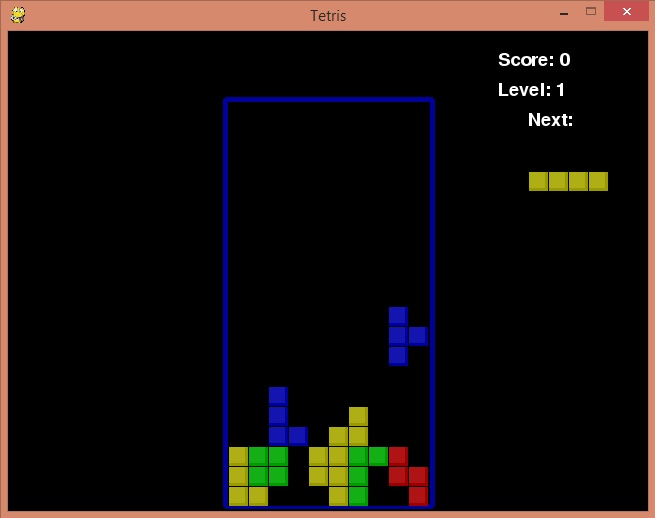
\includegraphics[width=2.9in]{board.jpg}
	\caption{Example of the game world}
	\label{Figure 1}
\end{figure}
\FloatBarrier

We consider a game called Tetris. Tetris is 2D game world where users stack blocks in order to make complete rows of blocks (complete rows disappear). The user receives a score point for each row cleared and loses if the stack of blocks reaches the top of the board. There are seven block shapes that are presented to the user for stacking.
The user can then decide to move the piece to the left or right, rotate it and then place it. 

\FloatBarrier
\begin{figure}[!h]
	\centering
	
\includegraphics[width=2.9in]{blocks.jpg}
	\caption{The different types of blocks a user is presented with and its associated label}
	\label{Figure 2}
\end{figure}
\FloatBarrier

We suggest collecting data of 3 different behaviours of a user playing Tetris. Each behaviour has a corresponding skill level indicated by how many lines can be cleared before losing. We have created three behaviour types with which to play the game:
\begin{itemize}
\item \textbf{Unskilled:} An agent that places blocks on the lowest point of the board with an average of lines cleared.
\item \textbf{Moderate:} An agent that minimizes the amount of empty spaces and places pieces in stacks with an average of 2 lines cleared.
\item \textbf{Skilled:} A human player that simply filled the board from left to right with an average of 26 lines cleared.
\end{itemize}
Then using the data created by these player we have created corresponding MDPs to represent each behaviour. Using these MDPs we create a new Tetris game called Adaptive Tetris that monitors the users actions in order to predict the users behaviour. Changes are then made to the game in order improve performance based on behaviour.
We suggest two phases to implement this: the training phase (where the MDPs are created) and the adaptive phase (which checks user behaviour and determines whether changes made are beneficial).
\subsection{    Phase 1: Data collection}

\begin{algorithm}
\caption{Training Phase}\label{euclid}
\begin{algorithmic}[1]
\Procedure{Create MDP ($\tau $)}{}
\State $\textit{MDP =} \phi$

\BState \emph{While Game Running}:
\State $\text{Observe the action made by the agent } \tau $
\State $\text{and then record the state, action }$
\State $\text{and the resultant state \{ s,a,s' \} }$
\State $\text{ in the set \{ S,A,S' \} }$

\BState \emph{for s in S}:
\State $\text{Update each action set with the}$
\State $\text{ probability P(a } |s,  \tau \text{) accordingly }$
\State $\text{MDP[s] = A}$
\EndProcedure
\end{algorithmic}
\end{algorithm}


Every user that plays Tetris has a skill level $\tau \in [0,2]$, where 0 represents Unskilled, 1 Moderate and 2 Skilled. With each skill level there is an associated probability $p \in [0,1]$ that the current agent corresponds to that skill level. There is also a probability that an agent will make an action given the state $P(a |s, \tau  ) \in [0,1]$. Our training phase is given as Algorithm 1. The algorithm runs indefinitely until shut down in order to create as much data as possible. Firstly allow the training user to play the game. After each action is made, record the action and the state of the game as well as the resultant state. In Tetris, the user can chose from the following actions: [Left, Right, Up, Down, Space, NoAction]. The state of the game is represented by the height of each column and the block's position, shape and rotation. [0,0,2,2,3,4,5,12,15,3 L 0 3 4] is an example of a possible state. 

\subsection{    Phase 2: Adaptive algorithm}
\begin{algorithm}
\caption{Adaptive Algorithm}\label{euclid}
\begin{algorithmic}[1]
\Procedure{Adaptive game ($ \tau $)}{}
\State $\text{Set the probability for each agent}$
\State $\text{to be equally likely}$
\State $\text{Probabilites = [1/numAgents,...]}$
\BState \emph{While Game Running}:
\State $\text{Get a, r and s at t}$
\State $\text{Get all possible s and r }$
\State $\text{after taking action a at state s} $
\State $\text{ and call these s1:k and r1:k}$
\State $\text{Observe the action made by the agent } \tau $
\State $\text{Compute B'}$
\State $\text{B(t+1) = B(t) - B'}$
\State $\text{Update Probabilities:}$
\If $\text{if B(t+1) is empty then}$
\State $\text{B(t+1) = S(k)}$
\EndIf
\State $\text{Set A(t+1) = X(B(t+1))}$
\State $\text{t = t + 1}$
\State $\text{Calculate: logP(} \tau | \text{a) = logP(a} | \tau \text{) + logP(} \tau )$
\If {$ \text{any Probabilities  } \tau \approx 1 $} 
\State $\text{Make changes to game based on probabilities}$
\EndIf
\EndProcedure
\end{algorithmic}
\end{algorithm}

We initially set the likelihood to be equal for each agent $\tau $ such that it is equally possible the user is any agent. Then while the game is running we observe each action made and fetch the probability of the action from each MDP. We then update the probabilities for each agent. If the probability that the user is a particular agent reaches some threshold such as 98\% then we change the content based on which agent the user is likely to be. In the Tetris game we change the probability of certain pieces dropping as well as the fall frequency of the blocks based on what skill level the user is determined to be. For example: an unskilled player will get more squares and the fall frequency will drop to allow for more thought at block placement. The skilled player would be presented with a greater drop frequency and random blocks. The adaptive algorithm has only been applied after a threshold has been reached for a number of reasons. Firstly, we do not want to present content to a user that is incorrect for that user. Secondly, by allowing the content to be presented after a certain threshold we can be certain that the content is meant for that user. This has the added benefit that if the probability goes below the threshold then we can remove the adaptive content till we are certain again that the user is of a certain type.

\section{Experiment}

We ran three experiments with each of the three users. In each experiment, we had each user type play the game Adaptive Tetris. The game was essentially the same for each experiment. However, we recorded different types of data to help us understand three important questions: 
\begin{itemize}
\item Are we correctly able to identify a user?
\item Is the time it takes to identify the user reasonable?
\item Does the adaptive algorithm improve user performance?
\end{itemize}

\subsection{    Results}

\subsection*{Accuracy}
\FloatBarrier
\begin{figure}[!h]
	\centering
	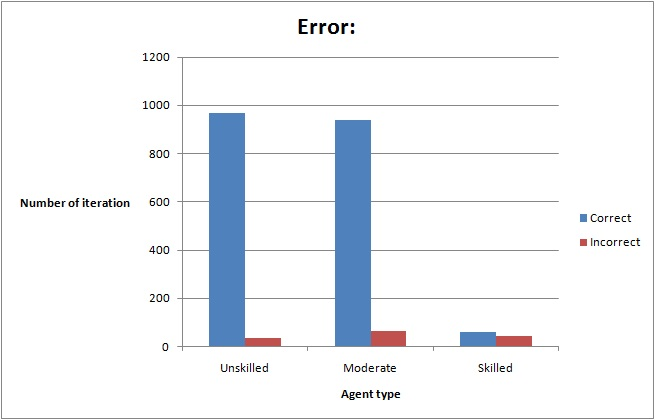
\includegraphics[width=3in]{accuracy.jpg}
	\caption{The accuracy at predicting each type}
	\label{Figure 3}
\end{figure}
\FloatBarrier
\FloatBarrier
\begin{figure}[!h]
	\centering
	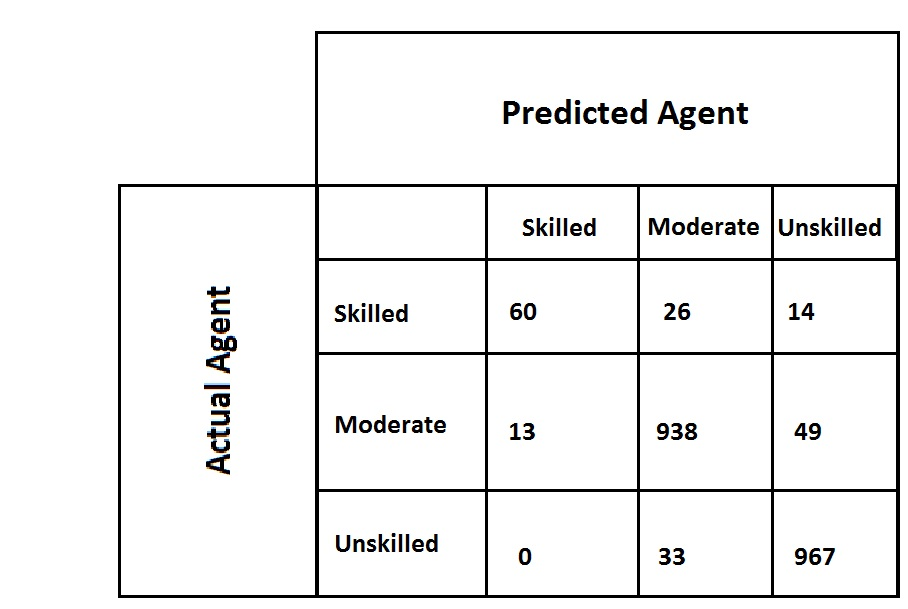
\includegraphics[width=3in]{confuse.jpg}
	\caption{Confusion matrix of predictions}
	\label{Figure 2}
\end{figure}
\FloatBarrier
We ran the adaptive algorithm 1000 times for each agent and 100 times for the Skilled player. We found that the Unskilled agent was easy to identify, with 97\% of the guesses correctly identifying the agent. The Moderately skilled agent was also easy to identify with an accuracy of 94\%. However, the Skilled human player was more difficult to identify, with only 70\% of the guesses being made correctly. We interpret that the Skilled player made actions that could be found in either of the other two agents action set. Since a skilled player in Tetris does not necessarily follow a single distinguishable behaviour but rather makes use of many.
Overall, the algorithm made correct guesses as to the identity of the unskilled and moderate players with distinct behaviour 95\% of the time. A representative confusion matrix is included to illustrate this.





\subsection*{Convergence time}
\FloatBarrier
\begin{figure}[!h]
	\centering
	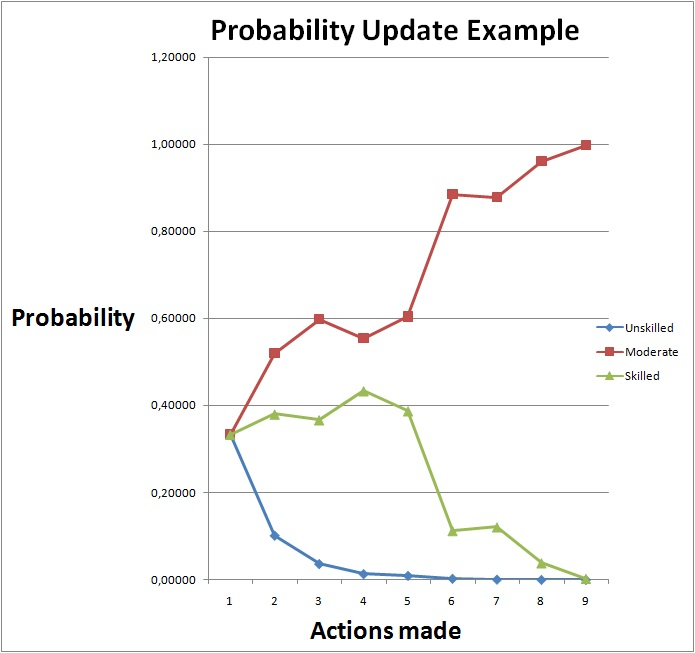
\includegraphics[width=3in]{eg.jpg}
	\caption{Example of probabilities converging}
	\label{Figure 4}
\end{figure}
\FloatBarrier

To calculate the time it took to predict agent type, we simply recorded how many steps were required to make a prediction. Since an action made corresponds to an update in the algorithm, we can instead refer to how many actions the user had to make. We recorded the actions taken in the same manner as we did when finding accuracy. However, the actions taken for each agent differed wildly without any real pattern. This can be attributed to the fact that an agent may make an action indicative of one agent then make another indicative of another, causing the probabilities to fluctuate. We noticed that sometimes the user could make 6 actions before a prediction was made and sometimes 400 actions could be made before a prediction was made. These times were in now way unique to each agent. So, we have rather taken an average prediction time from all the above data which we recorded as 38 actions from a set of 2100 games.


\subsection*{User Performance}
\FloatBarrier
\begin{figure}[!h]
	\centering
	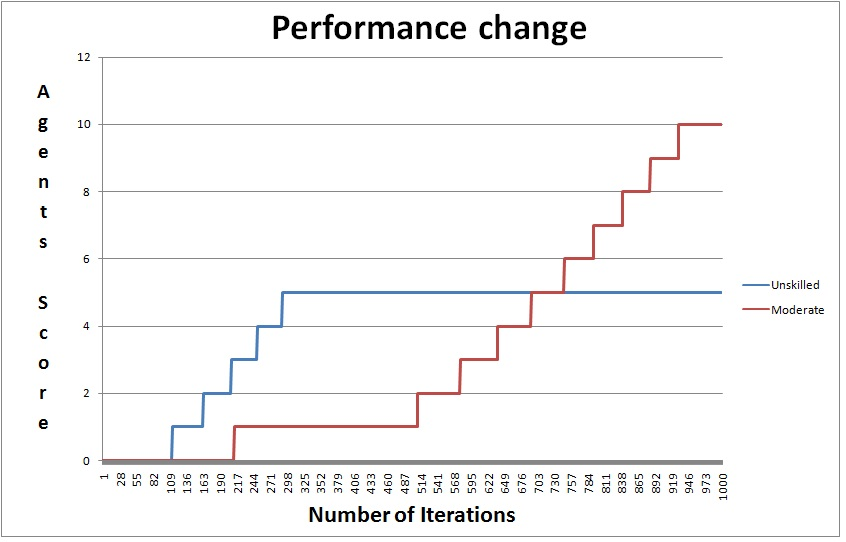
\includegraphics[width=3in]{s.jpg}
	\caption{The Average score of the agents several games}
	\label{Figure 5}
\end{figure}
\FloatBarrier
We first calculated the average score of each player type by observing all the games they played for the training phase of the MDPs. We calculated that the average score for a skilled player was 26 lines cleared, 0 lines for the unskilled and 2 lines cleared for the moderately skilled player. Using this we can directly check to see if any of the adaptations made in the game improve player score. To adapt the game we changed the type of pieces given to them and changed the block fall frequency. As before we ran the game 1000 times for each agent and 100 times for the skilled player. We found that in 71\% of the games played by the moderate and unskilled players score was above the average for his behaviour type. The performance of the skilled player decreased due to the adaptive game making the game more difficult for the skilled players.


\subsection{   Discussion}
Future work can be done into refining this method into a more robust method. That can be implemented quickly and effectively into other situations. Situations such as basic software and perhaps web-development could see use of this algorithm in their implementation. Existing game developers could make use of it on a broader scale by incorporating it into existing games titles. Altogether, the algorithm has a wide range of uses in computing and could possibly reach many markets. As such, all these factors contribute to us thinking of it as a highly sophisticated approach to the way developers present content to their users and as such we see it as a viable research topic.

As we noted, the algorithm had a difficult time pointing out the Skilled player since its behaviour could be seen in the other two agents. The current experiments could be conducted on agents of ambiguous behaviour. This would be done to see how we could split similar behaviours apart from one another so as to make the algorithm more accurate.


\section{Conclusion}

This paper presented a method to identify user type so that we could provide individualised content to that user. In this paper we explored the use of MDPs as a novel approach at developing adaptive computer games. We provided an algorithm that can be used to generate MDPs representing user types. We also provided an algorithm with which to interpret these MDPs and provide appropriate changes based on this. This method was based on an existing method \cite{ramamoorthy2013latent} to determine user type.  We then showed the viability of this algorithm in providing content to the user through the use of three experiments in the Tetris domain. In which we were correctly able to identify user types in real time and then provide the users with individualised content. The possibilities regarding future work based off of this algorithm are many. As we have shown, there are a multitude of ways in which this algorithm could be used in real world applications. We hope that further work will be done in implementing the algorithm in more complex systems with a larger array of diverse users thus showing the algorithm efficiency.



\newpage
\bibliographystyle{IEEEtran}
\bibliography{IEEEabrv,references}

\end{document}


